
\documentclass[aspectratio=169]{beamer}
\usepackage[english]{babel}
\usepackage[utf8x]{inputenx}
\usepackage{multicol} % indice en 2 columnas
\usepackage{subfig}
\usepackage{tikz-timing}[2009/05/15]
\usepackage{enumerate} % enumerados
\usepackage{wrapfig} %preámbulo
%\usepackage{pstricks}
\usepackage{textpos}
\usepackage{csvsimple}

\usetheme{CambridgeUS}
\usecolortheme{seahorse}
%\useoutertheme{shadow}
%\useinnertheme{circles}

\setbeamersize{text margin left=25pt,text margin right=25pt} 


\title[GraspJ]{GraspJ - GPU-Run Analysis for STORM and PALM in ImageJ}

\subtitle{AFIB - ICFO}

\author[Ismael Benito]{\bigskip \small Ismael Benito Altamirano}
\date[AFIB - ICFO]{\small \today}

\AtBeginSection{
\begin{frame}
  \frametitle{Index}
  \tableofcontents[currentsection] 
\end{frame}
}

\begin{document}

%\begin{frame}
%\maketitle
%\end{frame}

\addtobeamertemplate{frametitle}{}{%
\begin{textblock*}{110mm}(.65\textwidth,-1,25cm)

\includegraphics[height=1.5cm]{./images/logos.pdf}
\end{textblock*}}

\frame{\titlepage}

\begin{frame}
  \frametitle{Index}
  \tableofcontents
\end{frame}

\section{Introducing GraspJ}

\begin{frame}
\frametitle{Introducing GraspJ}

\begin{columns}[c]

\column{0.45 \textwidth}

 

\begin{figure}[h!]
    \centering	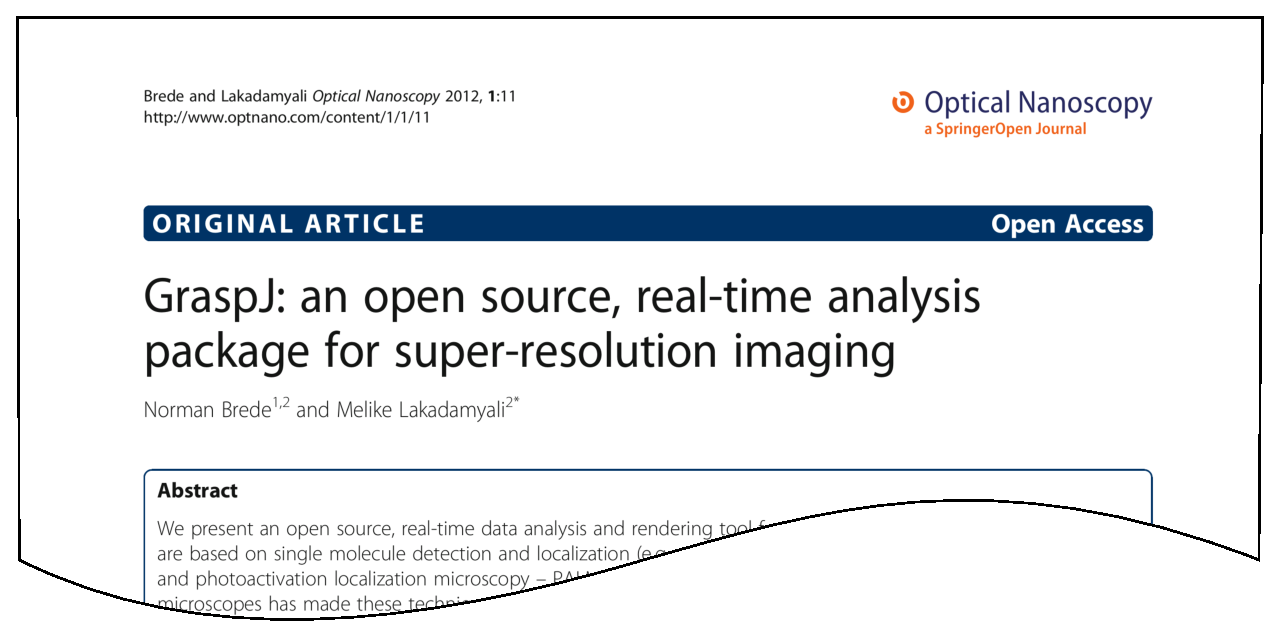
\includegraphics[width=\textwidth]{./images/graspj_paper.pdf} 
    %\caption{}
    %\label{fig:use}
    \end{figure} 

\textbf{GraspJ: an open source,real-time analysis package for super-resolution imaging}  \\  
Norman Brede and Melike Lakadamyali    

\column{0.55\textwidth}

Was developed by Norman Brede at AFIB as his master thesis. It is thougth:

\begin{itemize}
 \item As a plugin of ImageJ or FIJI.
 \item To be able to run in a GPU based system.
 \item To be able to run in realtime with Labview.  
 \item To be open source.
\end{itemize}



\end{columns}
    
    
\end{frame}


\subsection{Dependencies \& Modes}

\begin{frame}
\frametitle{Dependencies \& Modes}

\begin{columns}[c]


\column{0.75\textwidth}

\textbf{Dependencies}

\begin{itemize}
 \item \emph{Java Virtual Machine (JVM):} needs at least Version 7. 
 \item \emph{OpenCL:} Open Computing Language, allows the possibility to compute in GPUs. Needs compiler and Drivers. 
\end{itemize}

\textbf{Modes}

\begin{itemize}
 \item \emph{Standalone Mode:} Runs indepently from ImageJ/FIJI. Less realtime features. Easier to run. 
 \item \emph{Plugin Mode:} Runs inside ImageJ/FIJI. More realtime features. JVM versions issues.  
\end{itemize}

\column{0.15 \textwidth}

 

\begin{figure}[h!]
    \centering	
\includegraphics[width=0.9\textwidth]{./images/java.png} \\
    \centering	
\includegraphics[width=0.9\textwidth]{./images/OpenCL.png} \\
    \centering	
\includegraphics[width=0.9\textwidth]{./images/fiji.jpg} 
    %\caption{}
    %\label{fig:graspj1}
\end{figure} 


\end{columns}
\end{frame}


\subsection{Common use}
\begin{frame}
\frametitle{Common use}

\begin{figure}[h!]
    \centering	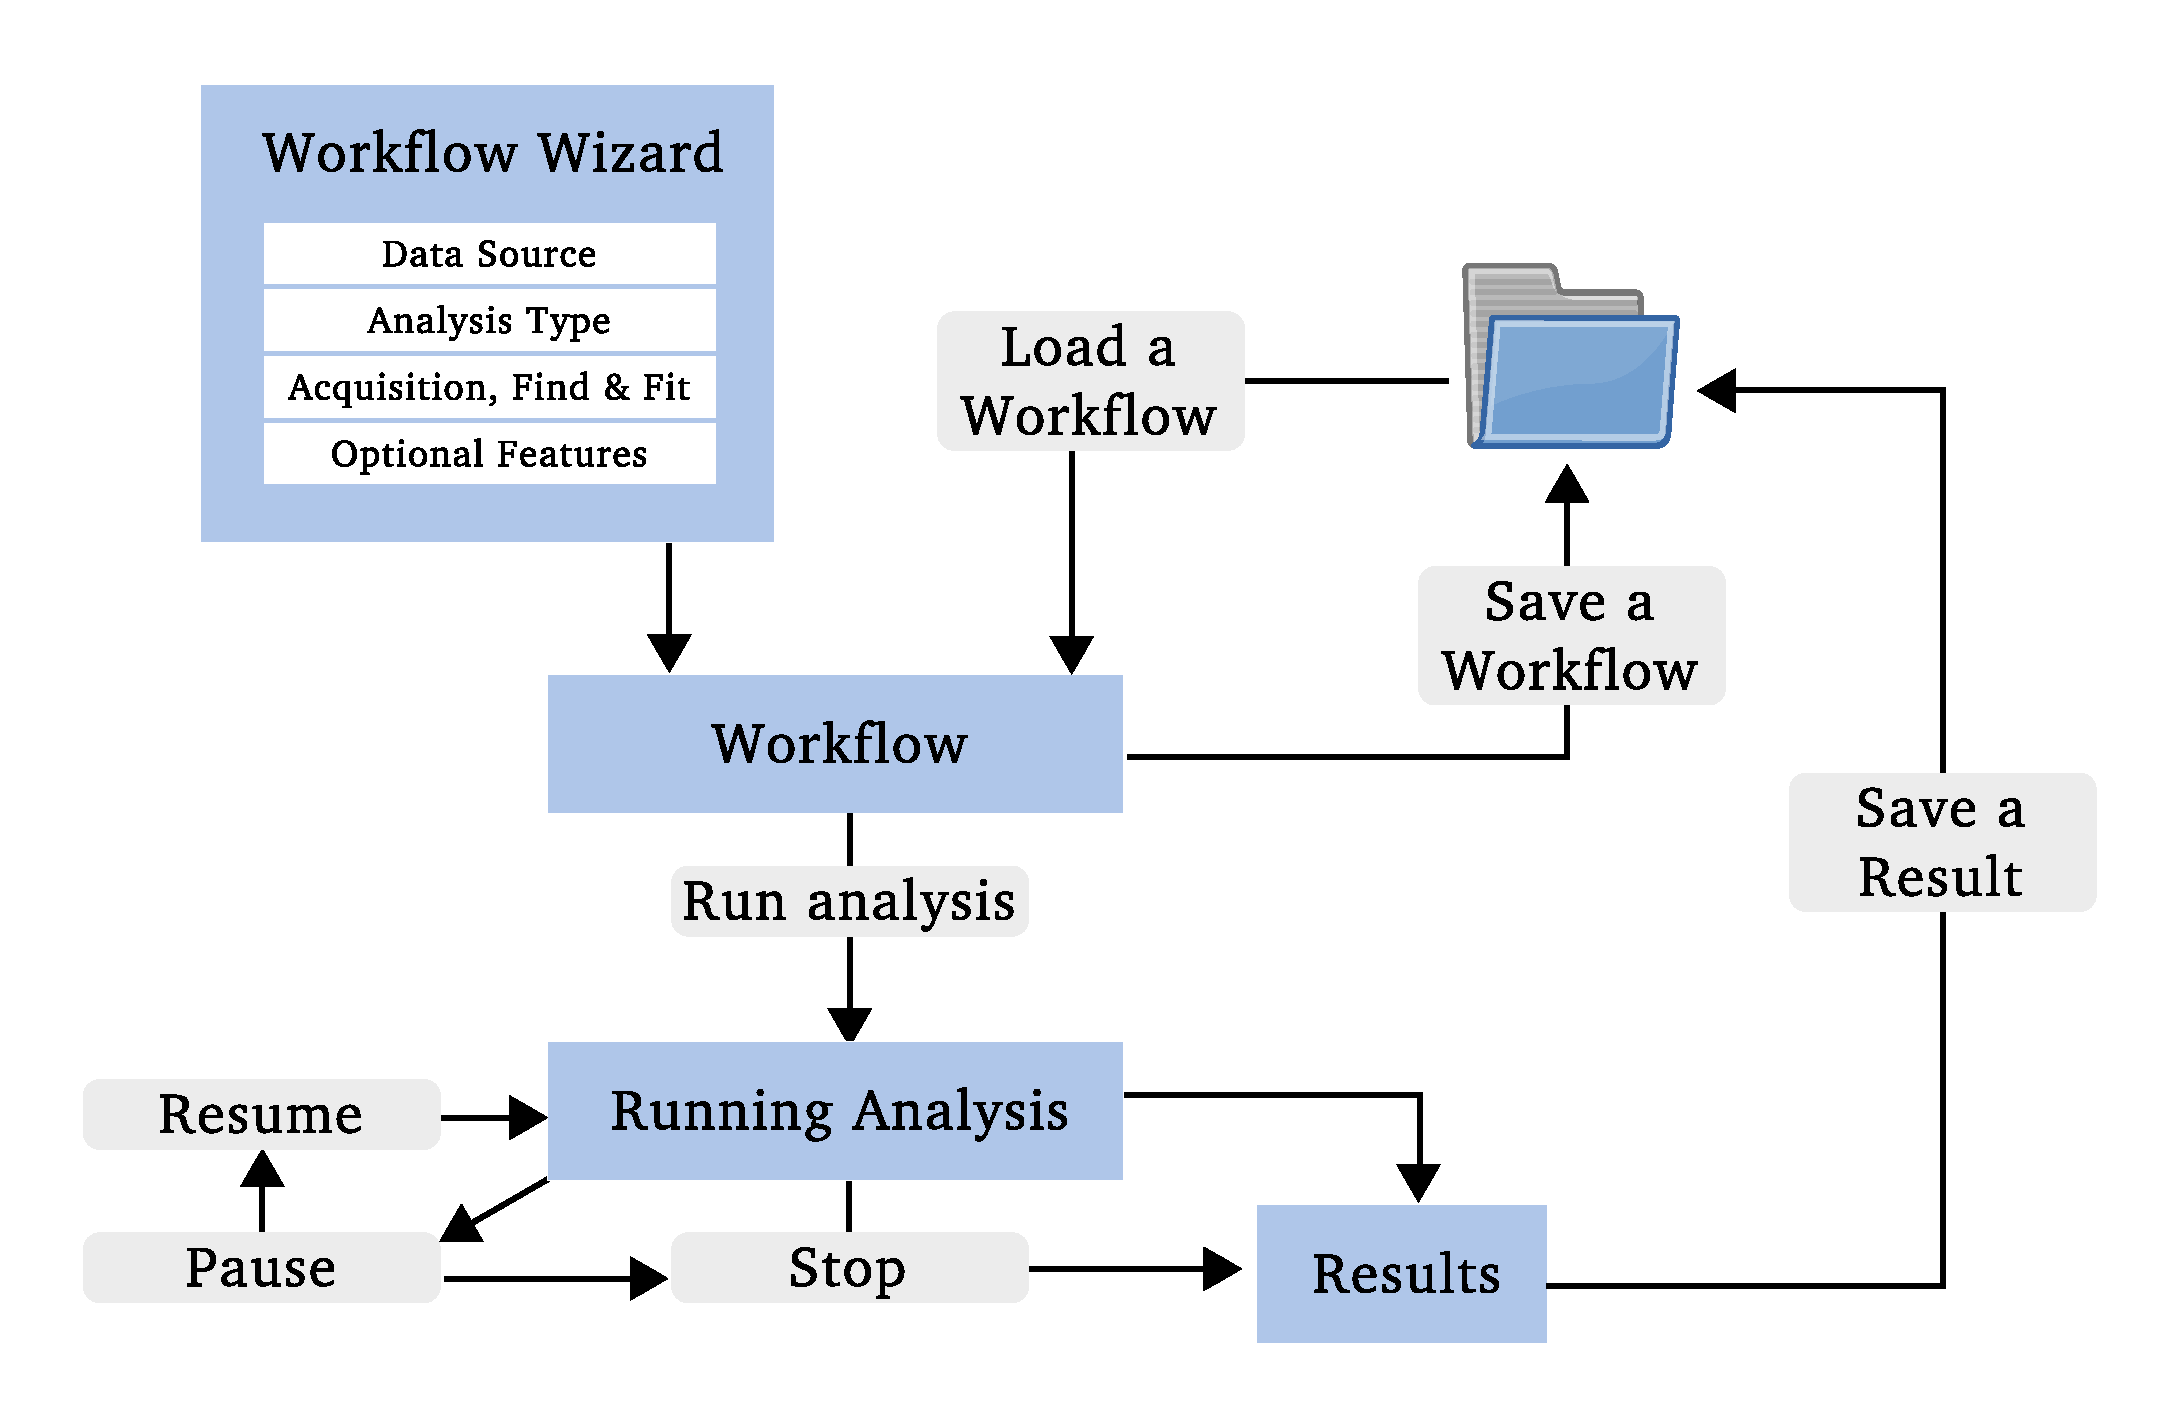
\includegraphics[width=0.75\textwidth]{./images/common_use.pdf} 
    %\caption{}
    %\label{fig:use}
    \end{figure} 
 
\end{frame}



\subsection{Workflow details}
\begin{frame}

\frametitle{Workflow details}

\begin{columns}


\column{0.33\textwidth}
    \begin{figure}
    \centering	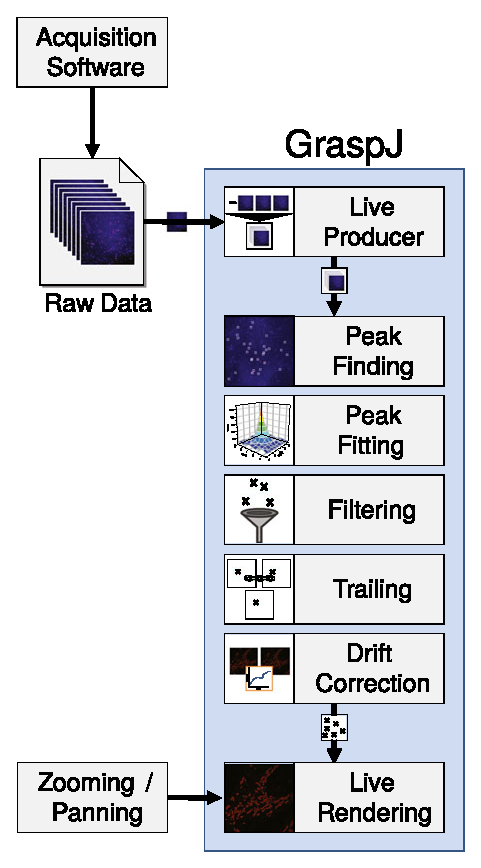
\includegraphics[trim=0cm 0.5m 0cm 0cm, clip, width=0.6\textwidth]{./images/workflow.pdf} 
    %\caption{}
    %\label{fig:use}
    \end{figure} 
    
    \emph{\tiny Norman Brede and Melike Lakadamyali.}

\column{0.66 \textwidth}

\begin{itemize}
 \item \emph{Live Producer:} creates the  packages of frames. 
 \item \emph{Peak Finding:} Peaks are identified based on a threshold.
 \item \emph{Peak Filtering:} Mean positions are determined
 \item \emph{Filtering:} Localizations resulting from peak fitting can be filtered.
 \item \emph{Trailing:} Peaks that appear in close proximity in consecutive frames are trailed together.
 \item \emph{Drift correction:} Drift is determined by phase correlating consecutive, temporally split high resolution images.
 \item \emph{Live Rendering:} Final localizations are rendered as Gaussians.
\end{itemize}    
    
    
\end{columns}

    
\end{frame}
    

\section{Fixing errors and features}

\subsection{Load Error}
\begin{frame}
\frametitle{Load Error}
\begin{figure}[h!]
    \centering	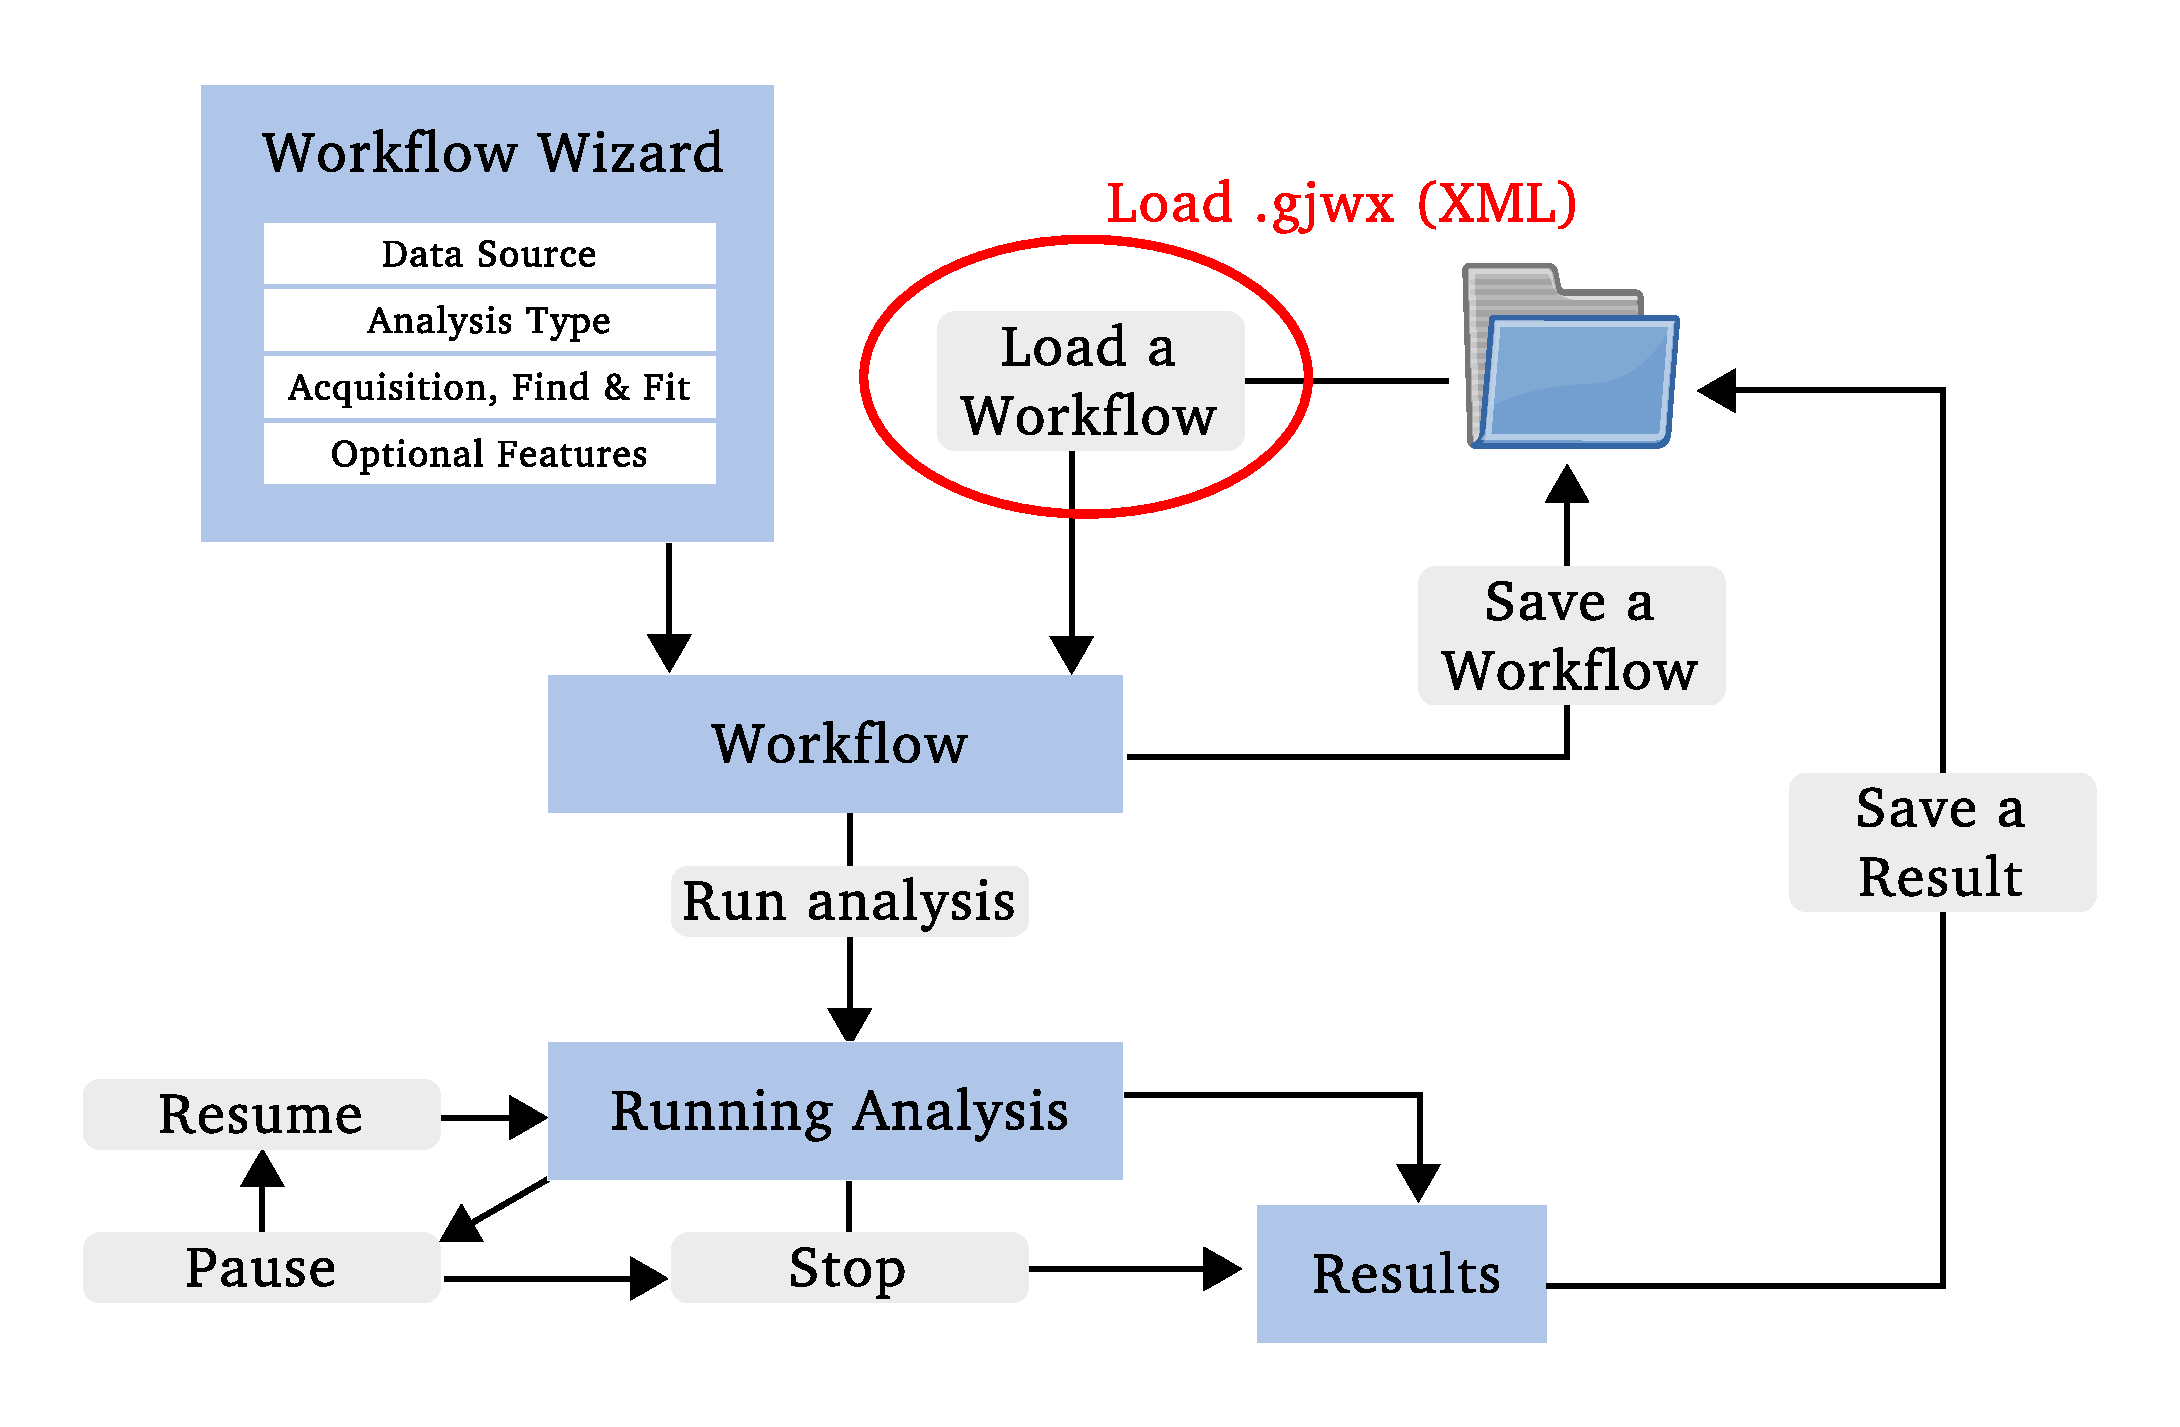
\includegraphics[width=0.75\textwidth]{./images/load_error.pdf} 
    %\caption{}
    %\label{fig:load_error}
    \end{figure} 
 
\end{frame}


\subsection{Result Error}
\begin{frame}
\frametitle{Result Error}
\begin{figure}[h!]
    \centering	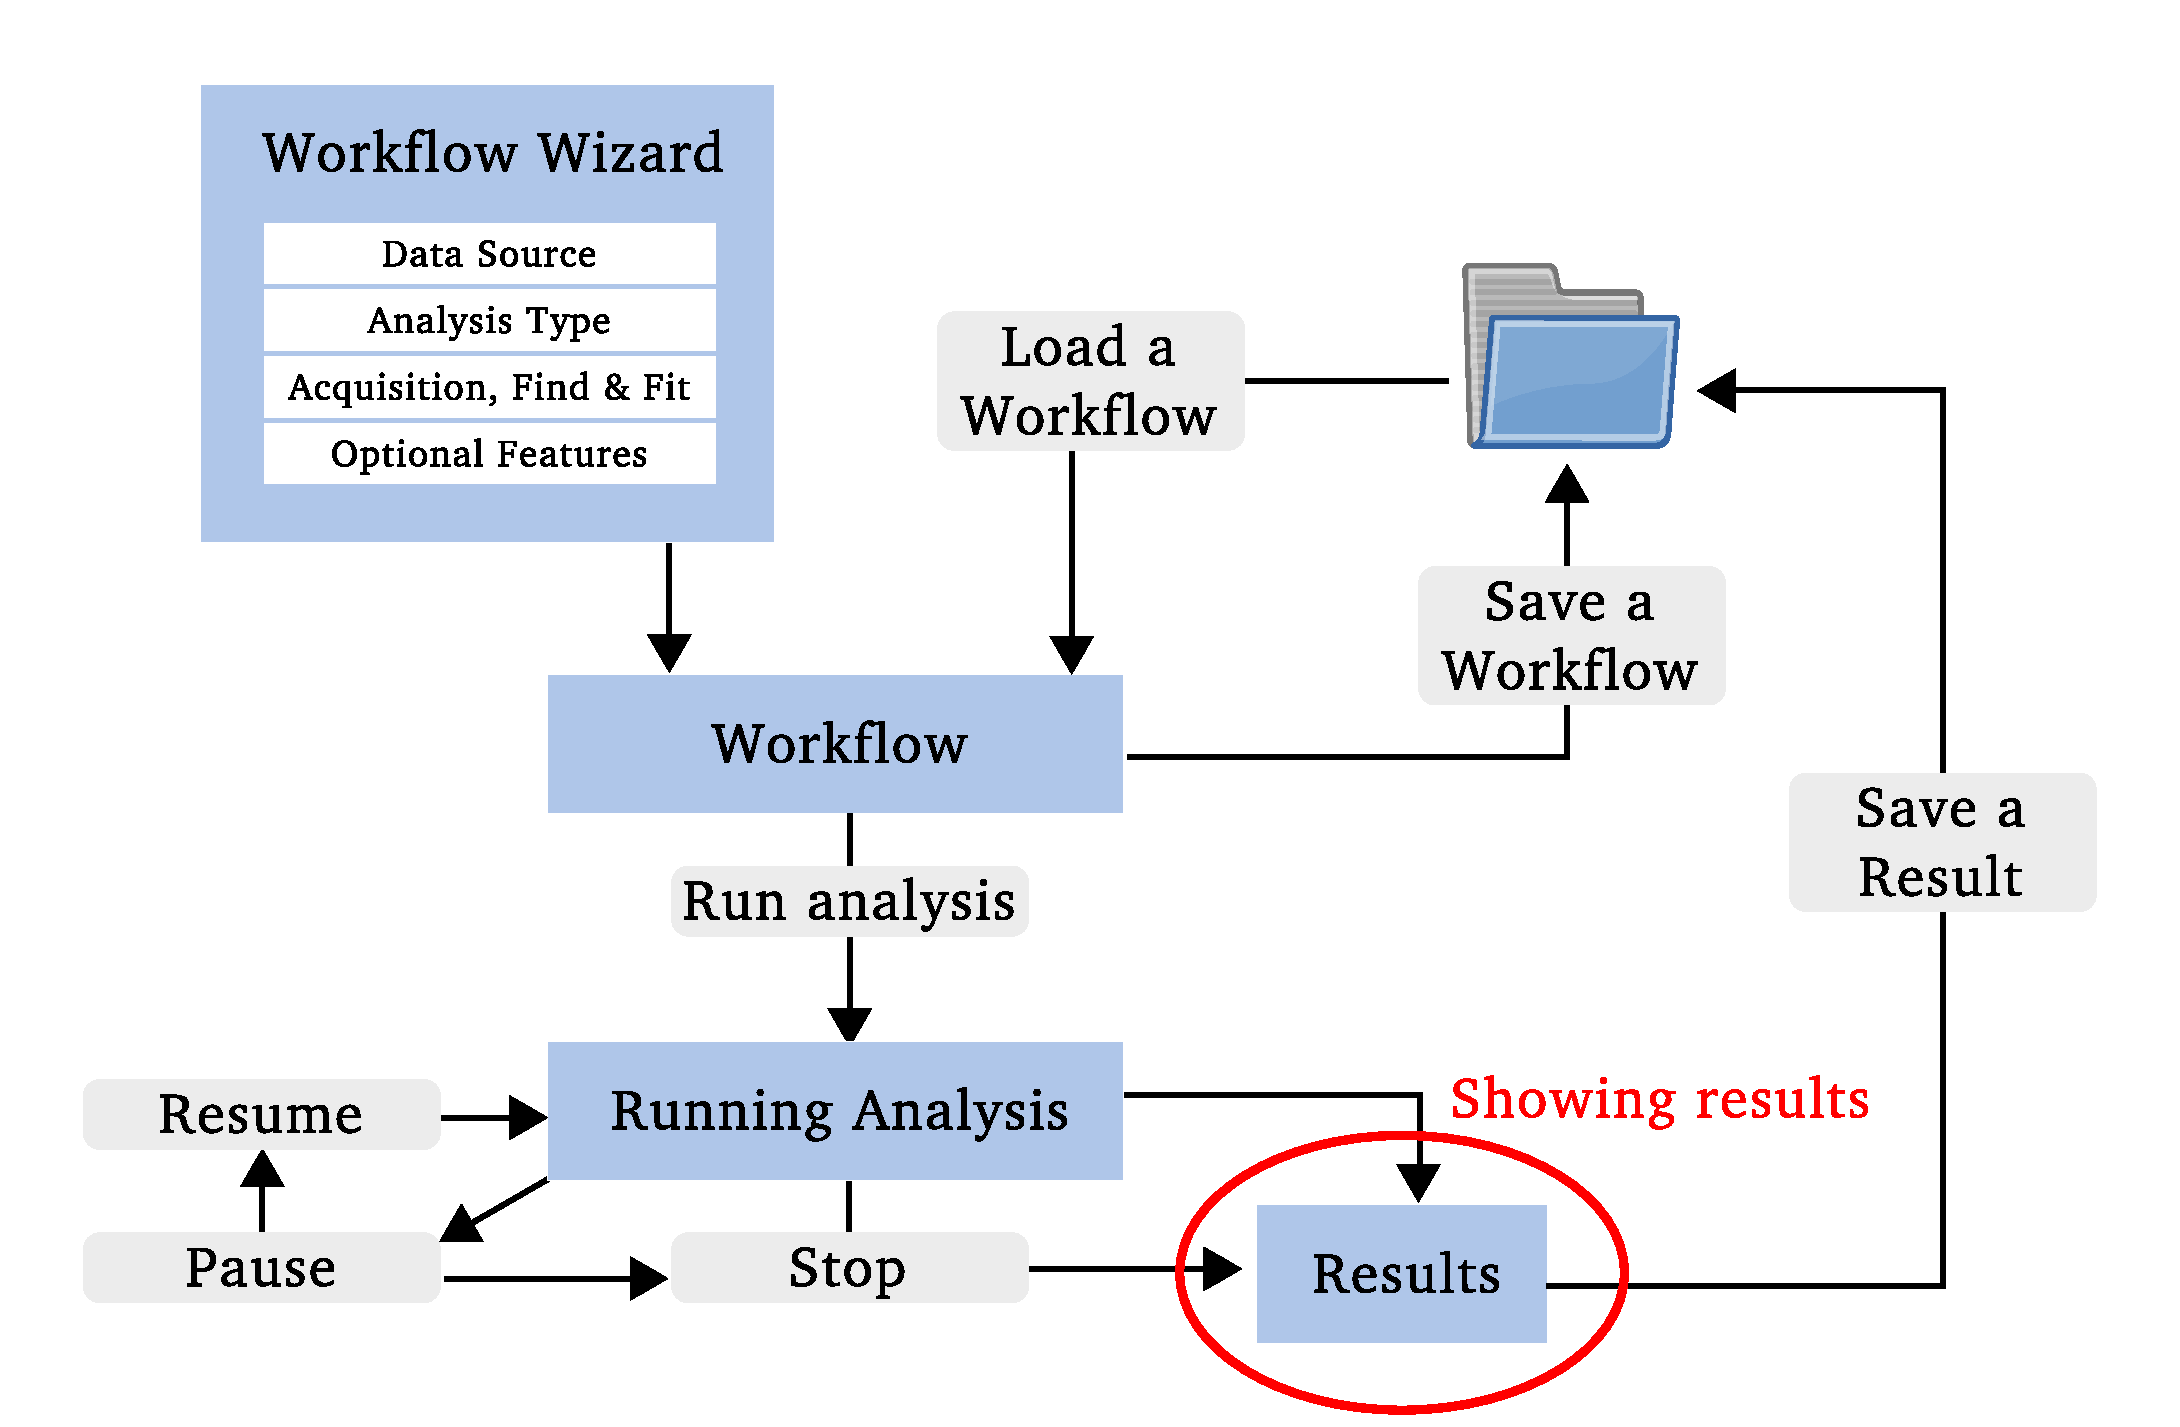
\includegraphics[width=0.75\textwidth]{./images/results_error.pdf} 
    %\caption{}
    %\label{fig:use}
    \end{figure} 
 
\end{frame}

\subsection{OpenCL Exception}
\begin{frame}
\frametitle{OpenCL Exception}
\begin{figure}[h!]
    \centering	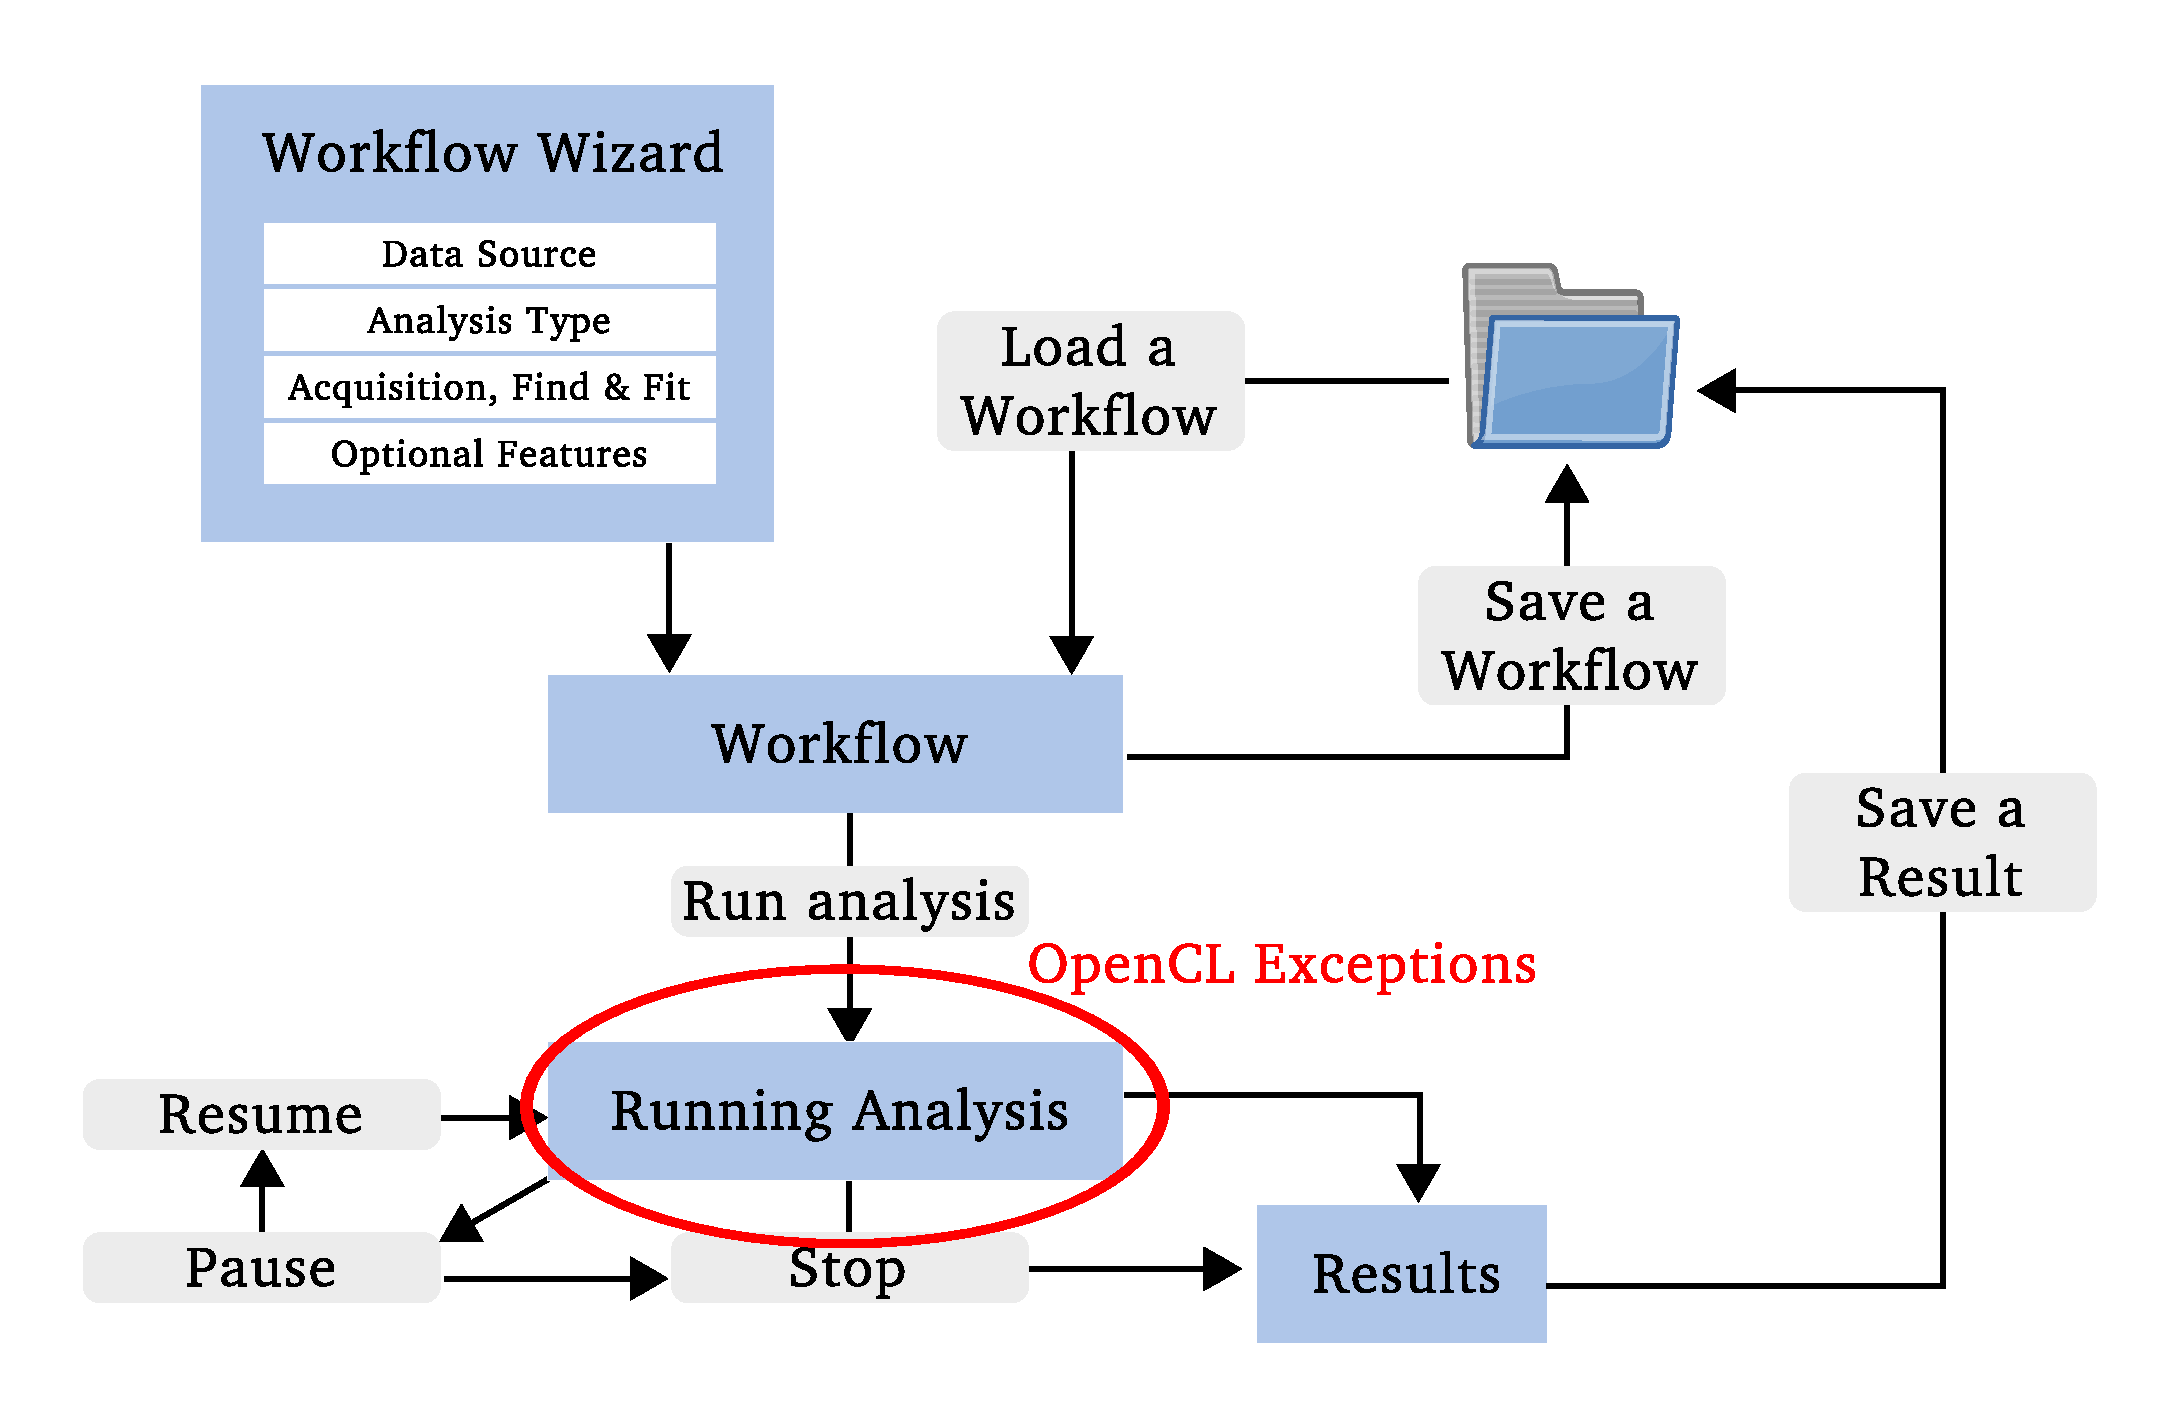
\includegraphics[width=0.75\textwidth]{./images/opencl_error.pdf} 
    %\caption{}
    %\label{fig:use}
    \end{figure} 
 
\end{frame}

\subsection{Workflow ``Mistake''}
\begin{frame}
\frametitle{Workflow ``Mistake''}
\begin{figure}[h!]
    \centering	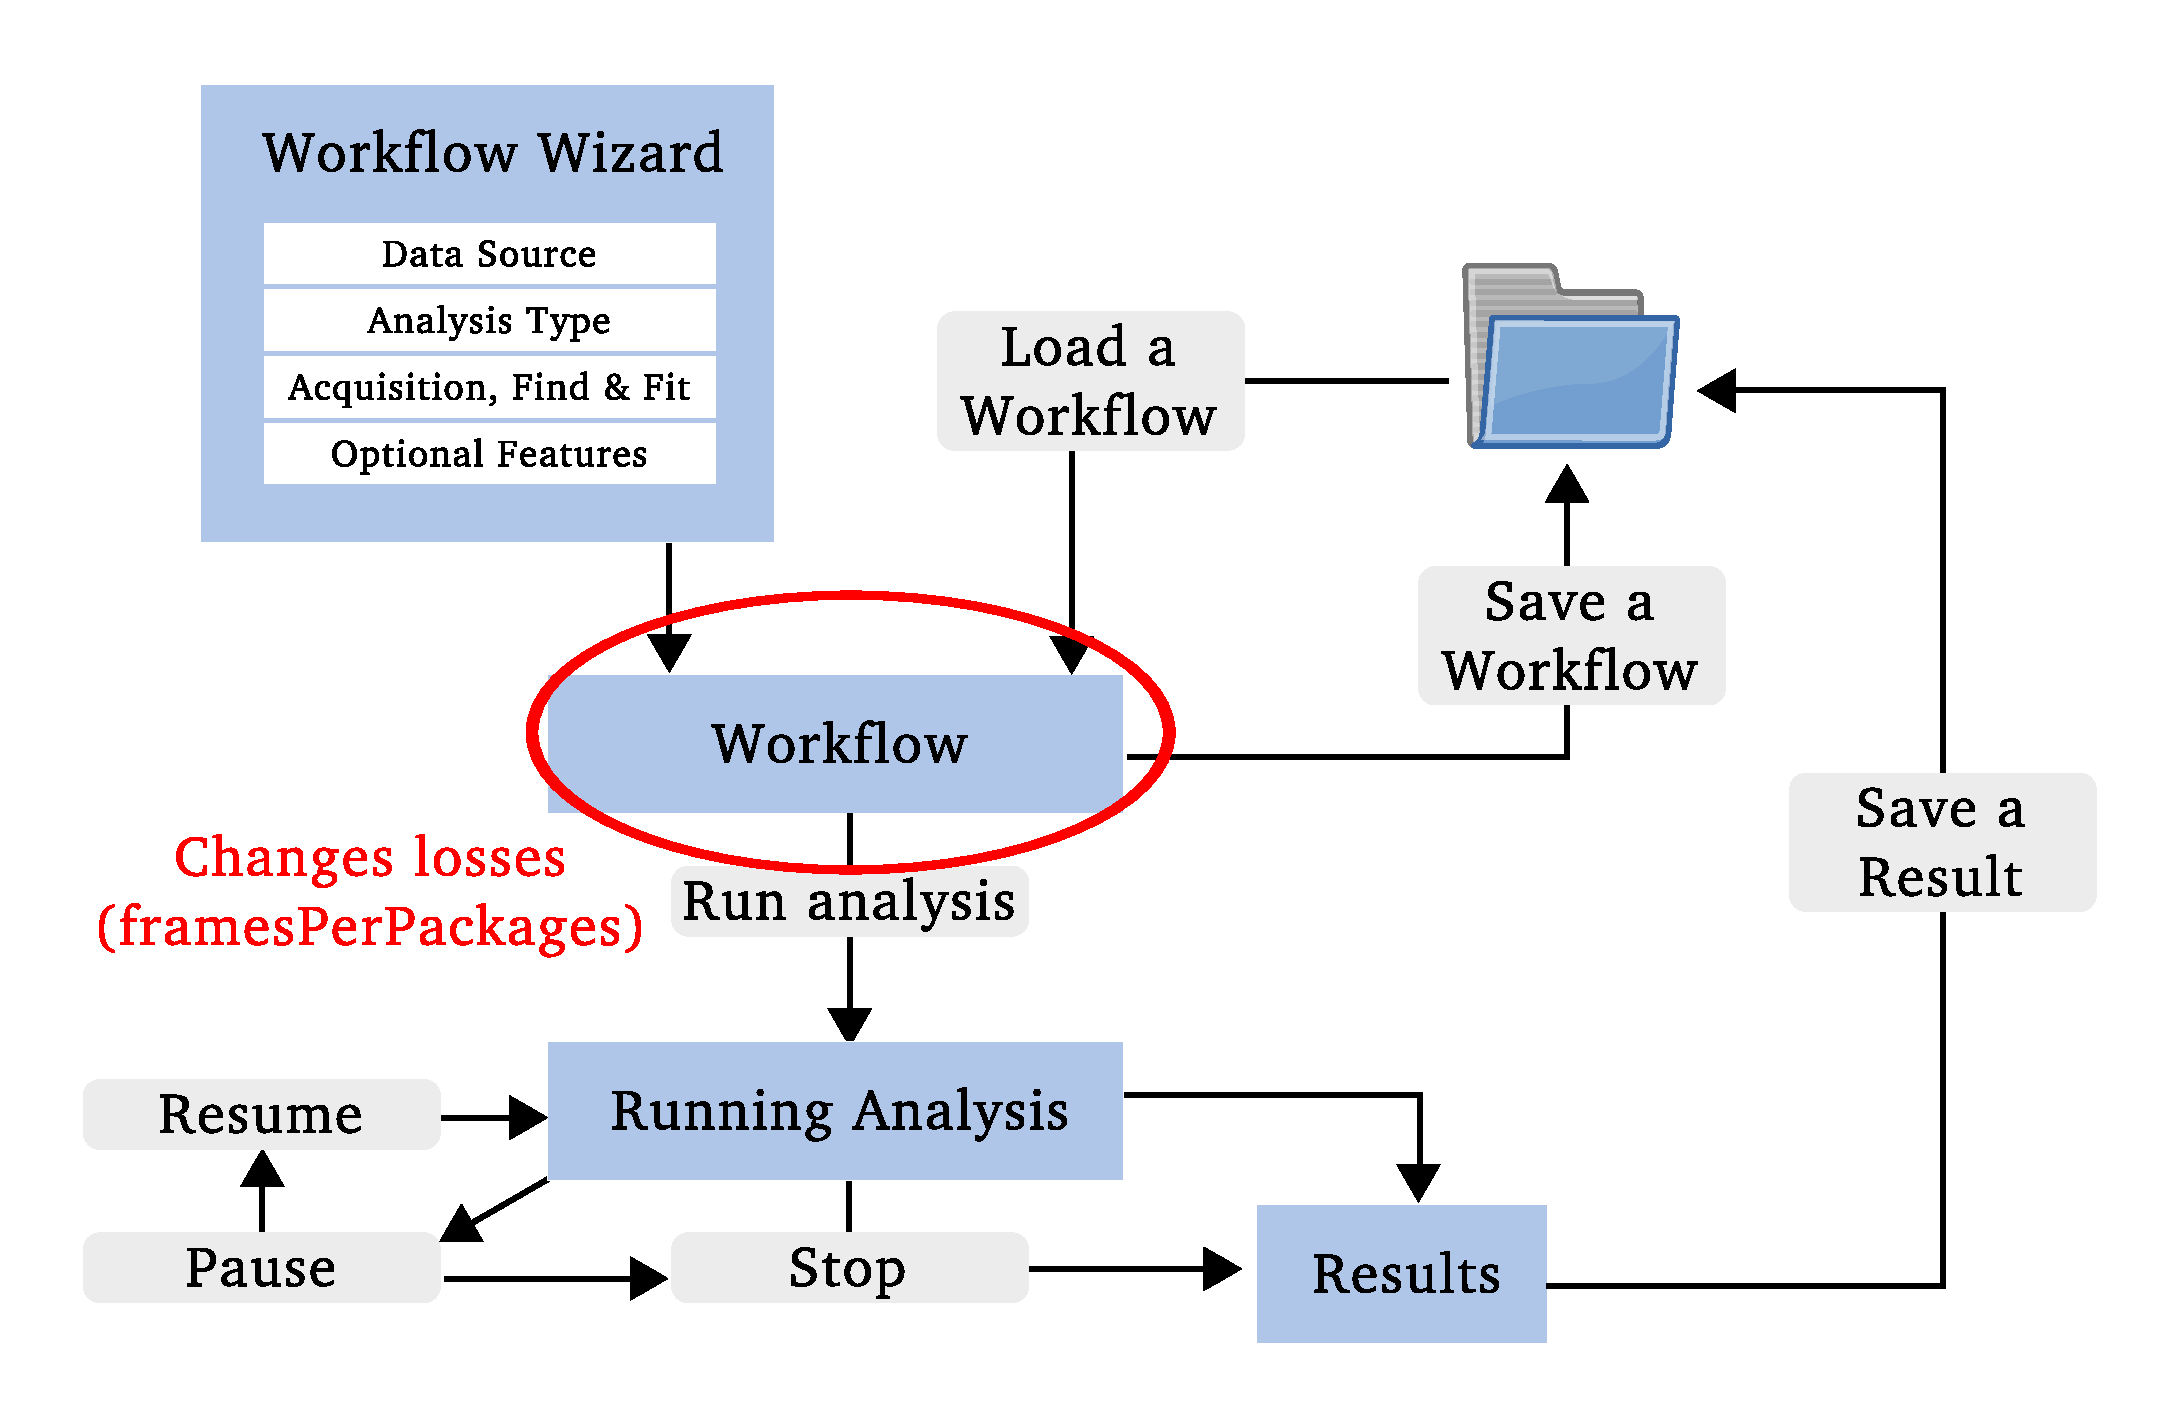
\includegraphics[width=0.75\textwidth]{./images/workflow_error.pdf} 
    %\caption{}
    %\label{fig:use}
    \end{figure} 

    
\end{frame}



\section{DAOSTORM}


\begin{frame}
\frametitle{DAOSTORM}

\begin{columns}[c]

\column{0.45 \textwidth}

 

\begin{figure}[h!]
    \centering	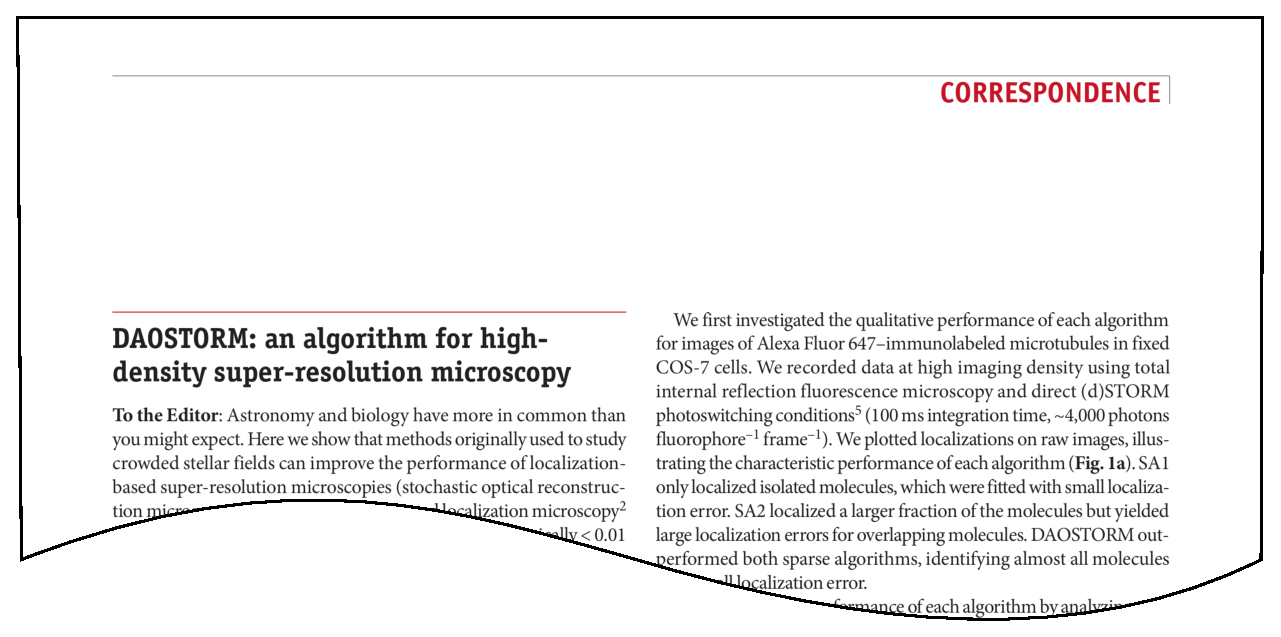
\includegraphics[width=\textwidth]{./images/dao_paper.pdf} 
    %\caption{}
    %\label{fig:use}
    \end{figure} 
    
\textbf{DAOSTORM: an algorithm for high-density super-resolution microscopy}  \\  
Seamus J Holden, Stephan Uphoff \& Achillefs N Kapanidis


\column{0.55\textwidth}

Was developed forking DAOPHOT II algotrithm from star detections. The basis of the algorithm are: 

\begin{figure}[h!]
    \centering	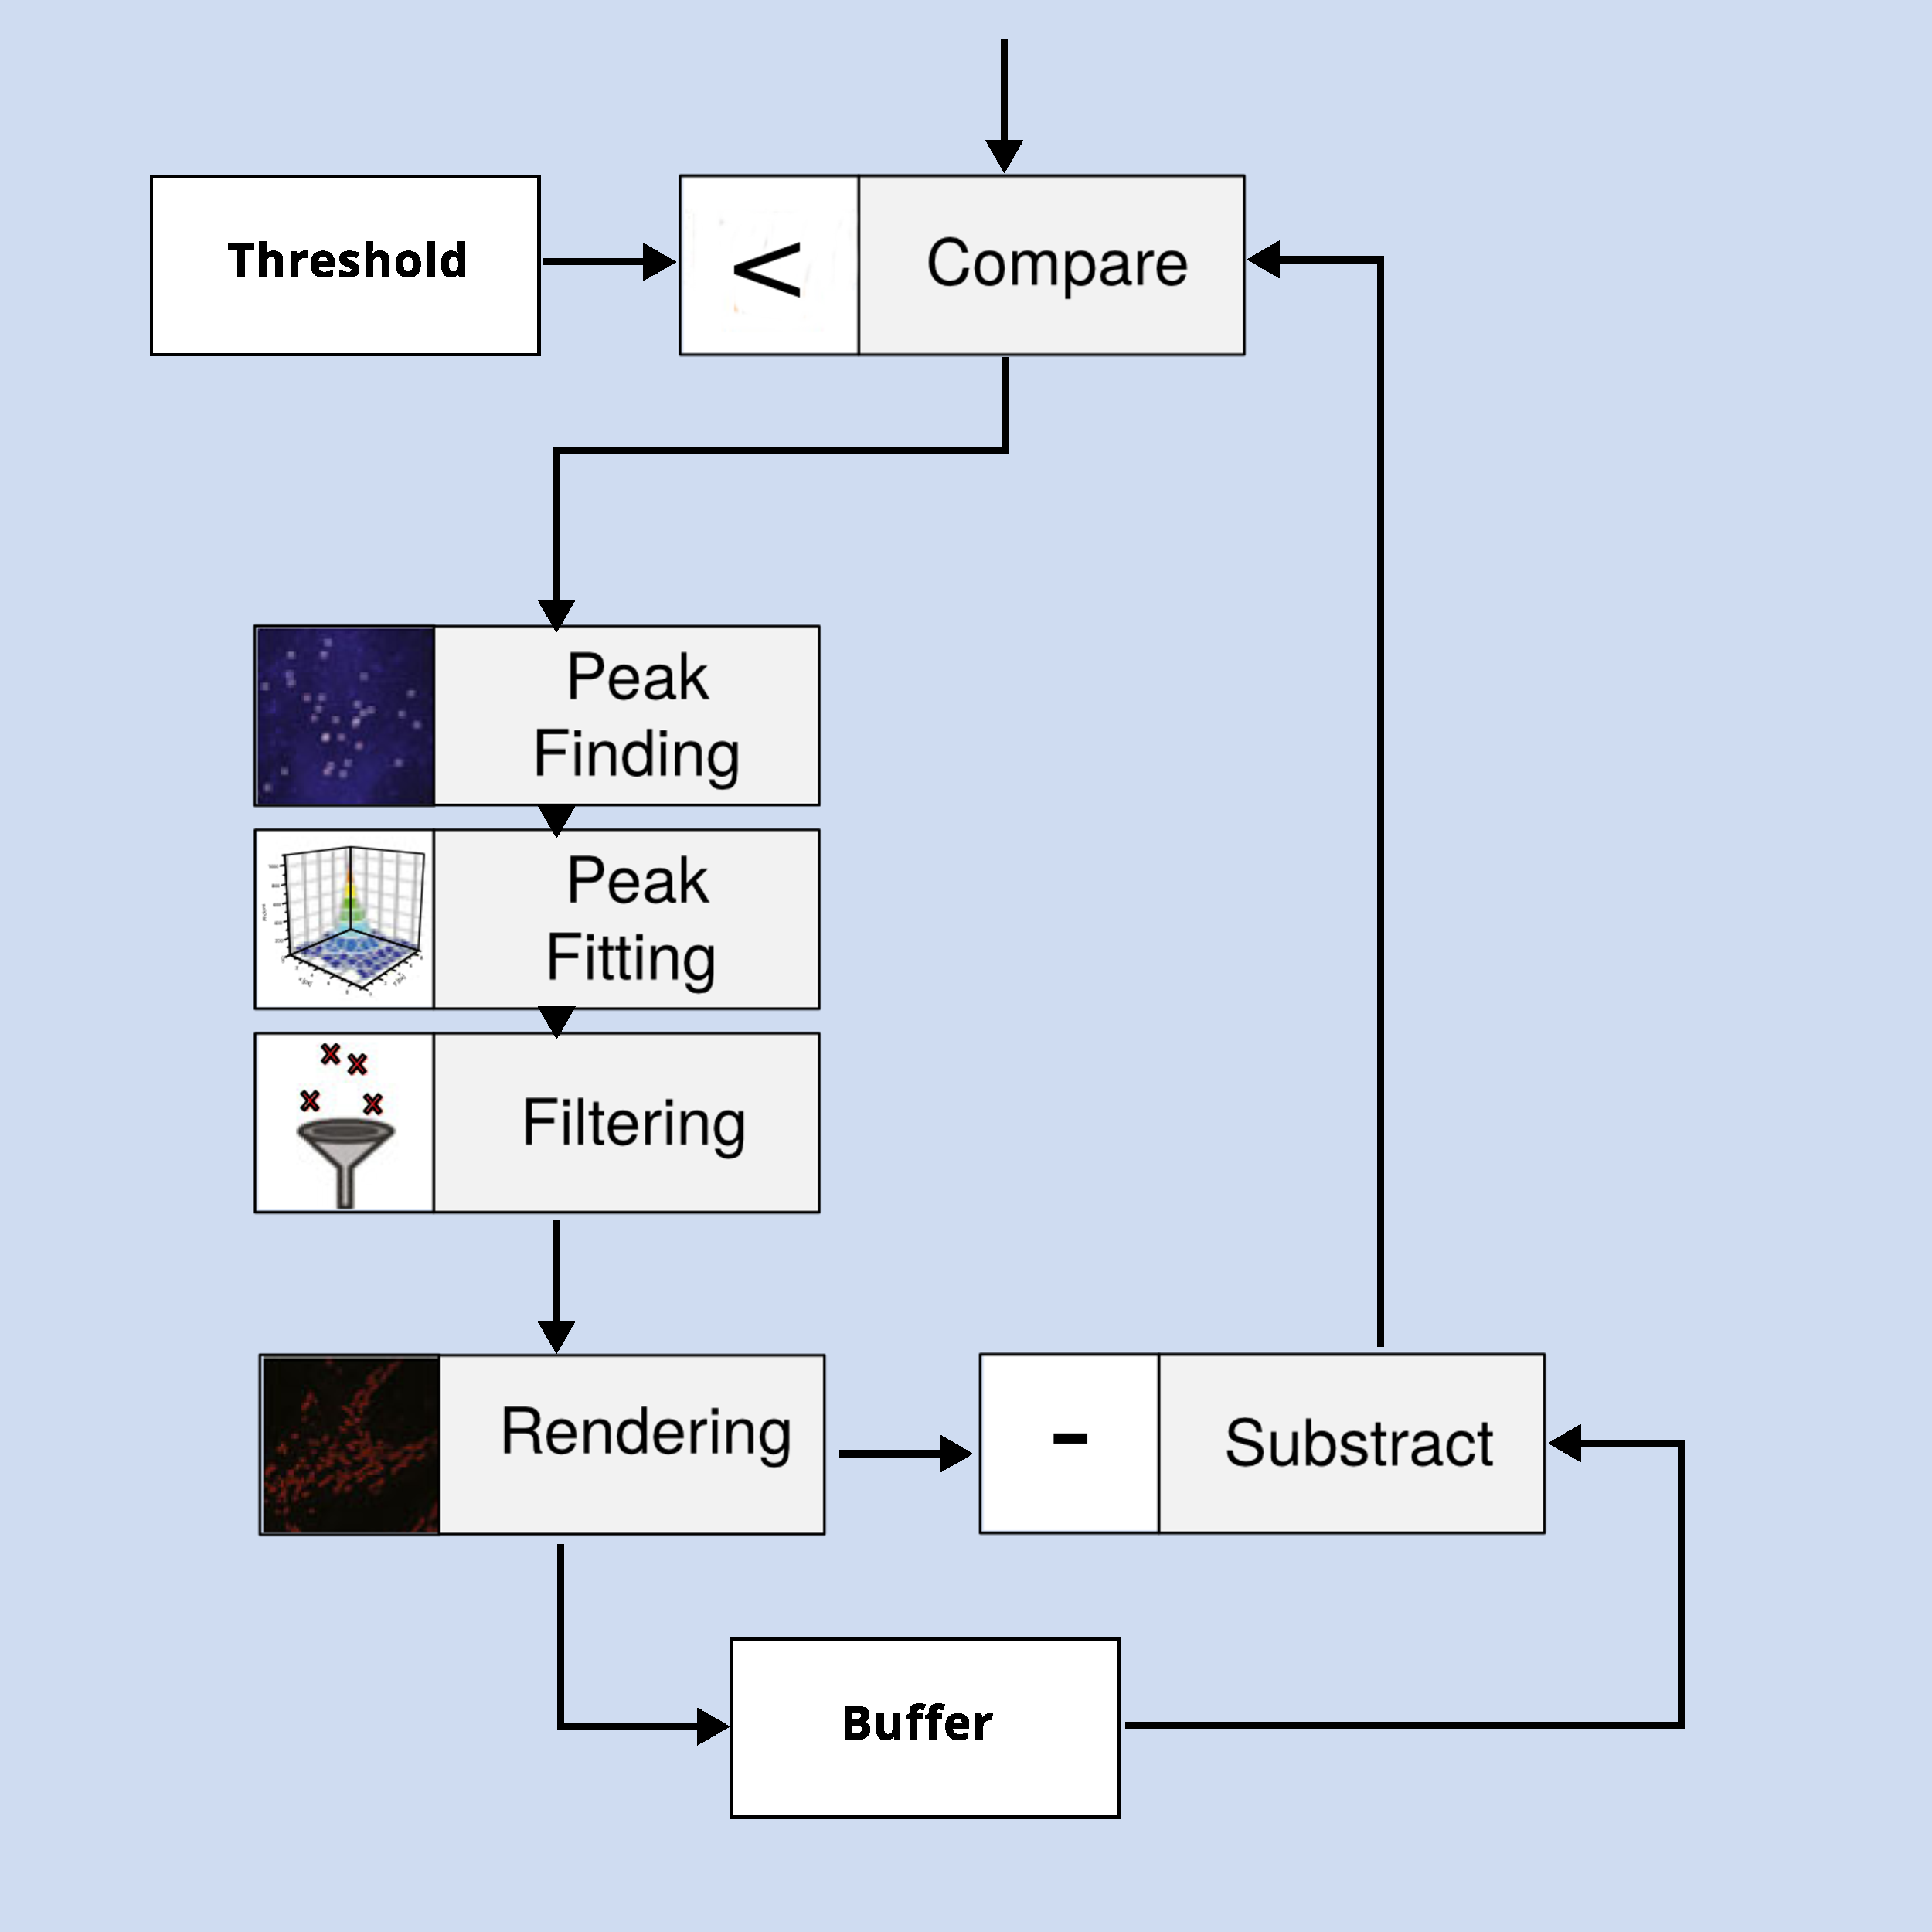
\includegraphics[width=0.6\textwidth]{./images/dao_workflow.pdf} 
    %\caption{}
    %\label{fig:use}
    \end{figure} 





\end{columns}
    
    
\end{frame}


\end{document}